% agenda-ajout-rdv.tex
\section*{Ajouter un rendez-vous}
\addcontentsline{toc}{section}{Ajouter un rendez-vous}
Pour créer un nouveau rendez-vous quelque soit le mode, il suffit de cliquer sur une quelconque date apparaissant dans le calendrier affiché, et la fenêtre suivante s'ouvrira, si la date correspond au jour du rendez-vous, autant cliquer directement dessus.
\begin{figure}
	\centering
	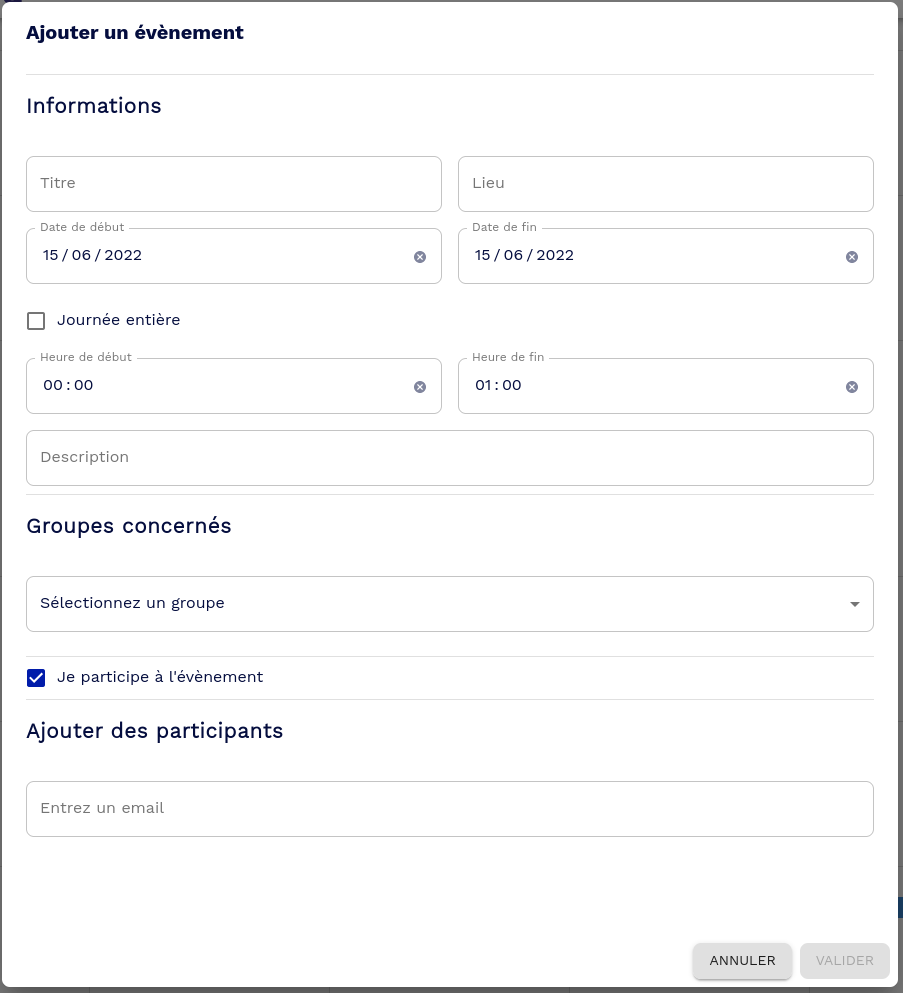
\includegraphics[width=0.500\linewidth]{./Captures/agenda.neo.rdv.png}
%	\caption{}
\end{figure}

Cependant, si vous êtes en mode hebdomadaire ou en mode journalier, et qu'avant de cliquer vous sélectionnez une plage horaire --dans cet exemple, on devine à gauche de la fenêtre de saisie du rendez-vous la sélection des plages allant du lundi 17h15 jusqu'à 19h par cette légère teinte bleuté ou verdoyante.
\begin{figure}
	\centering
	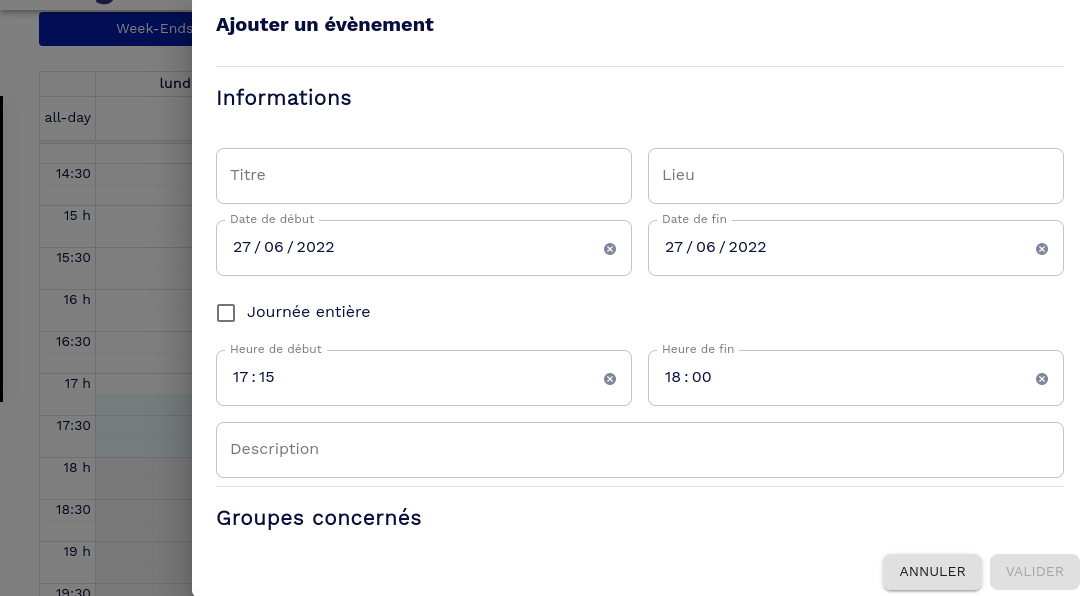
\includegraphics[width=0.500\linewidth]{./Captures/agenda.neo.rdv.selection.anterieure.png}
%	\caption{}
\end{figure}
Comme le montre la capture précédente, une partie des champs descriptifs du rendez-vous est saisie, voici le résultat lorsque tout est rempli (groupe associé, contacts supplémentaires concernés ajoutés)
\begin{figure}
	\centering
	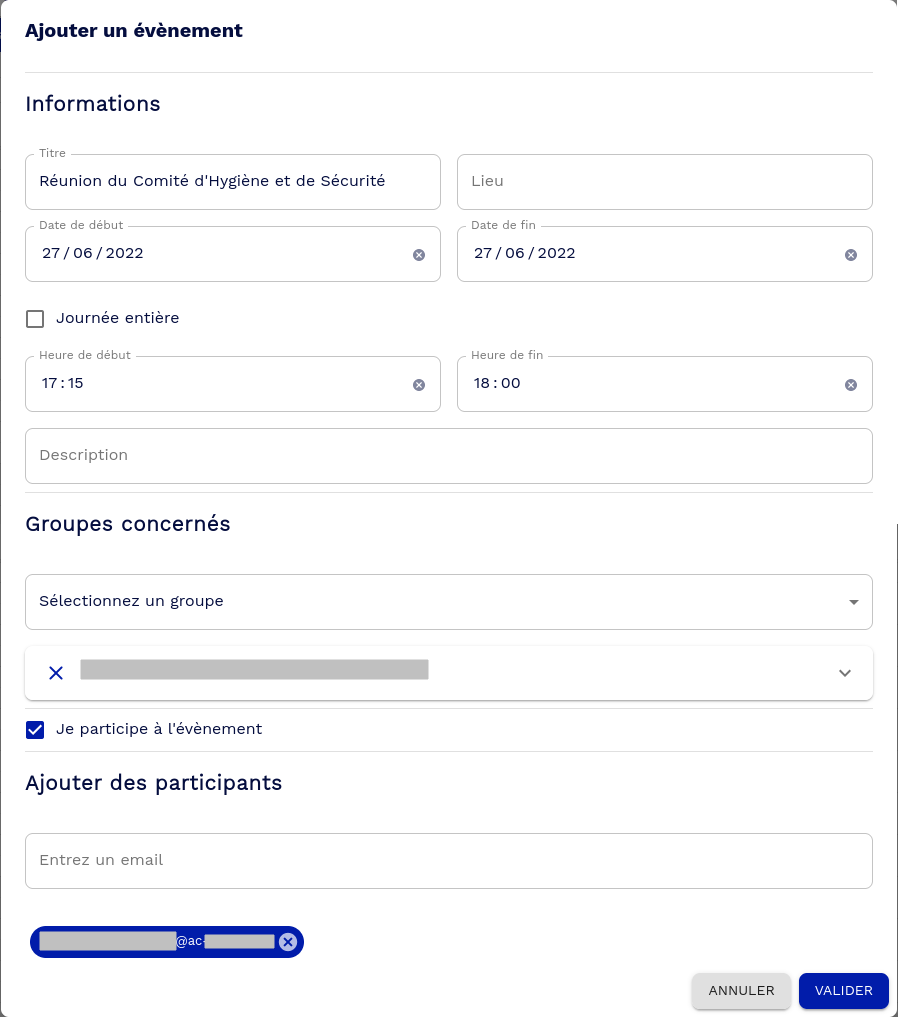
\includegraphics[width=0.500\linewidth]{./Captures/agenda.rendez.vous.exemple.complet.png}
	\caption{Un exemple complet de rendez-vous}
\end{figure}

Dès l'ajout, la notification --ici deux rendez-vous ont été ajoutés-- apparaît sur le portail, près de l'icône du profil.
\begin{figure}
	\centering
	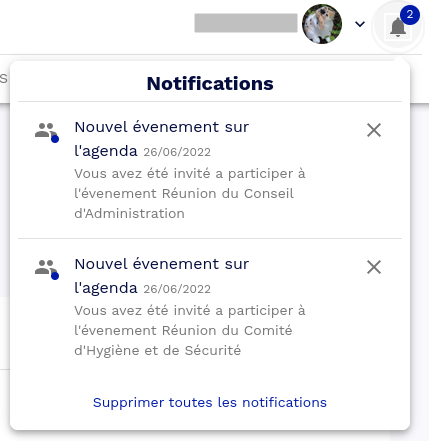
\includegraphics[width=0.500\linewidth]{./Captures/portail.agenda.notification.png}
	\caption{Notifications d'ajouts de nouveaux rendez-vous}
\end{figure}
et dans le groupe la vignette des événements fait apparaître le nombre d'événements
\begin{figure}
	\centering
	
\includegraphics[width=0.250\linewidth]{./Captures/agenda.affichage.evenement.dans.groupe.png}
%	\caption{}
\end{figure}
en cliquant dessus, les événements du groupe apparaissent par ordre décroissant des dates
\begin{figure}
	\centering
	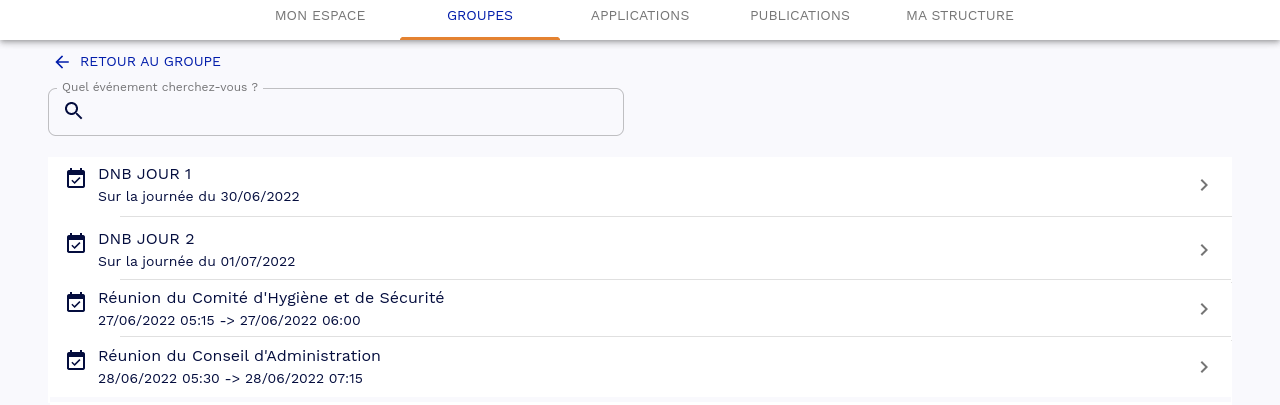
\includegraphics{./Captures/portail.groupe.evenements.details.png}
%	\caption{}
\end{figure}
l'appui sur le symbole ``~>~'' à droite de la ligne ouvrira un nouvel onglet en affichant les détails du rendez-vous.